\documentclass[12pt]{article}
\usepackage[top=1in, bottom=1in, left=.75in, right=.75in]{geometry}
\usepackage{amsmath}
\usepackage{fancyhdr}
\usepackage{graphicx, xcolor}
\usepackage{txfonts}
\usepackage{multicol,coordsys,pgfplots}
\usepackage[scaled=0.86]{helvet}
\renewcommand{\emph}[1]{\textsf{\textbf{#1}}}
\usepackage{anyfontsize}
% \usepackage{times}
% \usepackage[lf]{MinionPro}
\usepackage{tikz,pgfplots}
%\def\degC{{}^\circ{\rm C}}
\def\ra{\rightarrow}
\usetikzlibrary{calc}
\pgfplotsset{compat = newest}
\newcommand{\blank}[1]{\rule{#1}{0.75pt}}

\pgfplotsset{my style/.append style={axis x line=middle, axis y line=
middle, xlabel={$x$}, ylabel={$y$}}}

%axis equal

%yticklabels={,,} , xticklabels={,,}

% \setmainfont{Times}
% \def\sansfont{Lucida Grande Bold}
\parindent 0pt
\parskip 4pt
\pagestyle{fancy}
\fancyfoot[C]{\emph{\thepage}}
\fancyhead[L]{\ifnum \value{page} > 1\relax\emph{Math 251: Midterm 1}\fi}
\fancyhead[R]{\ifnum \value{page} > 1\relax\emph{Fall 2022}\fi}
\headheight 15pt
\renewcommand{\headrulewidth}{0pt}
\renewcommand{\footrulewidth}{0pt}
\let\ds\displaystyle
\def\continued{{\emph {Continued....}}}
\def\continuing{{\emph {Problem \arabic{probcount} continued....}}\par\vskip 4pt}


\newcounter{probcount}
\newcounter{subprobcount}
\newcommand{\thesubproblem}{\emph{\alph{subprobcount}.}}
\def\problem#1{\setcounter{subprobcount}{0}%
\addtocounter{probcount}{1}{\emph{\arabic{probcount}.\hskip 1em(#1)}}\par}
\def\subproblem#1{\par\hangindent=1em\hangafter=0{%
\addtocounter{subprobcount}{1}\thesubproblem\emph{#1}\hskip 1em}}
\def\probskip{\vskip 10pt}
\def\medprobskip{\vskip 2in}
\def\subprobskip{\vskip 45pt}
\def\bigprobskip{\vskip 4in}

\begin{document}
{\emph{\fontsize{26}{28}\selectfont Math F251\hfill
{\fontsize{32}{36}\selectfont Midterm 1}
\hfill Fall 2022}}
\vskip 2cm
\strut\vtop{\halign{\emph#\hskip 0.5em\hfil&#\hbox to 2in{\hrulefill}\cr
\emph{\fontsize{18}{22}\selectfont Name:}&\cr
\noalign{\vskip 10pt}
%\emph{\fontsize{18}{22}\selectfont Student Id:}&\cr
%\noalign{\vskip 10pt}
%\emph{\fontsize{18}{22}\selectfont Calculator Model:}&\cr
}}
%\hfill
%\vtop{\halign{\emph{\fontsize{18}{22}\selectfont #}\hfil& \emph{\fontsize{18}{22}\selectfont\hskip 0.5ex $\square$ #}\hfil\cr
%Section: & 001 (Jill Faudree)\cr
%\noalign{\vskip 4pt}
%         & 002 (Ryan Bridges)\cr
%\noalign{\vskip 4pt}
%         & 005 (Leah Berman)\cr}}
%
\vfill
{\fontsize{18}{22}\selectfont\emph{Rules:}}

You have 90 minutes to complete the exam. 

Partial credit will be awarded, but you must show your work.

You may have a single handwritten $3 \times 5$ notecard.

Calculators are not allowed. 


Place a box around your  \fbox{FINAL ANSWER} to each question where appropriate.

%If you need extra space, you can use the back sides of the pages.
%Please make it obvious  when you have done so.

Turn off anything that might go beep during the exam.

Good luck!
\vfill
\def\emptybox{\hbox to 2em{\vrule height 16pt depth 8pt width 0pt\hfil}}
\def\tline{\noalign{\hrule}}
\centerline{\vbox{\offinterlineskip
{
\bf\sf\fontsize{18pt}{22pt}\selectfont
\hrule
\halign{
\vrule#&\strut\quad\hfil#\hfil\quad&\vrule#&\quad\hfil#\hfil\quad
&\vrule#&\quad\hfil#\hfil\quad&\vrule#\cr
height 3pt&\omit&&\omit&&\omit&\cr
&Problem&&Possible&&Score&\cr\tline
height 3pt&\omit&&\omit&&\omit&\cr
&1&&12&&\emptybox&\cr\tline
&2&&16&&\emptybox&\cr\tline
&3&&8&&\emptybox&\cr\tline
&4&&8&&\emptybox&\cr\tline
&5&&14&&\emptybox&\cr\tline
&6&&12&&\emptybox&\cr\tline
&7&&15&&\emptybox&\cr\tline
&8&&15&&\emptybox&\cr\tline
%&9&&15&&\emptybox&\cr\tline
&Extra Credit&&5&&\emptybox&\cr\tline
&Total&&100&&\emptybox&\cr
}\hrule}}}

\newpage
\begin{enumerate}
%%%%%DEFINTION OF DERIVATIVE
\item (12 points)
	\begin{enumerate}
	\item State the definition of $f'(x),$ the derivative of the function $f(x).$
	\vspace{1in}
	\item Find the derivative of $f(x) = \sqrt{5-x}$  using the limit definition of the derivative. No credit will be awarded for using other methods.
	\end{enumerate}
\newpage

%%%%SKETCH DERIVATIVE FROM GRAPH OF FUNCTION
\item (16 points) Use the graph of $g(x)$, in the figure below, to answer the questions (a)-(g). The dashed lines in the figure represent asymptotes of the graph of $g(x).$ 
%%%%Begin FIGURE
\begin{center}
%%G
%\begin{tikzpicture}
%\begin{axis}[x=1cm,y=1cm,scale=0.6,xscale=1, thick, my style, xtick={-7,-6,...,8,9}, ytick={1,...,6,7,8},xmin=-7.9, xmax=10, ymin=-1.5, ymax=8, mark size=3.0pt, grid = major]
%\addplot[thick, dashed,<->] coordinates {(-4,-1.5) (-4,8)};
%\addplot[dashed, thick,<->] coordinates {(-7.5,6) (10,6)};
%\addplot[ultra thick, ->,domain=2:10, samples=100]{6-4/(x-1)};
%\addplot[ultra thick, domain=-4:2, samples=100]{3-0.5*(x)};
%\addplot[ultra thick, domain=-7.8:-4.17, samples=100,<->]{6+0.5/(x+4.1)};
%\node at (-7,7){\large{$g(x)$}};
%\draw[fill=black, thick] (-4,5) circle  (1.2 mm);
%\end{axis}
%\end{tikzpicture}
%\\

%%G
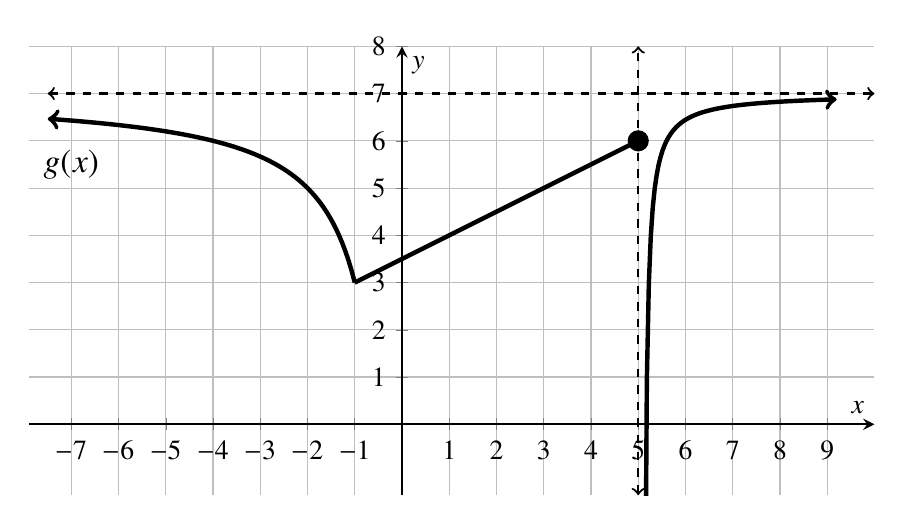
\begin{tikzpicture}
\begin{axis}[x=1cm,y=1cm,scale=0.6,xscale=1, thick, my style, xtick={-7,-6,...,8,9}, ytick={1,...,6,7,8},xmin=-7.9, xmax=10, ymin=-1.5, ymax=8, mark size=3.0pt, grid = major]
\addplot[thick, dashed,<->] coordinates {(5,-1.5) (5,8)};
\addplot[dashed, thick,<->] coordinates {(-7.5,7) (10,7)};
\addplot[ultra thick, <-,domain=-7.5:-1, samples=100]{7+4/(x)};
\addplot[ultra thick, domain=-1:5, samples=100]{3.5+0.5*(x)};
\addplot[ultra thick, domain=5.1:9.2, samples=100,<->]{7-0.5/(x-5.1)};
\node at (-7,5.5){\large{$g(x)$}};
\draw[fill=black, thick] (5,6) circle  (1.2 mm);
\end{axis}
\end{tikzpicture}
\\


%%G' location
\begin{tikzpicture}[scale=0.6]
\draw[->,thick](-8,0)--(10,0);
\draw[->,thick](0,-3)--(0,5);
\node at (9.5,.4){$x$};
\node at (0.4,4.5){$y$};
%\node at (-9,3){\large{$g'(x)$}};
\end{tikzpicture}
\end{center}
%%%% End FIGURE

\vfill

\begin{enumerate}
\begin{multicols}{2}
\item $\displaystyle{\lim_{x\to 5^-} g(x) = }$
\vfill
\item $\displaystyle{\lim_{x\to 5^+} g(x) = }$
\vfill
\item $\displaystyle{g(5)=}$
\vfill
\item $\displaystyle{\lim_{x\to -1} g(x) = }$
\vfill
\end{multicols}
\item Sketch the graph of $g'(x)$ on the axes below the graph $g(x).$ Label important points on the $x$ and $y$ axes.
\vspace{.4in}
\item For what $x$-values does the function $g(x)$ fail to be continuous?
\vfill
\item For what $x$-values does the \textbf{derivative} of $g(x)$, $g'(x)$, fail to be continuous?
\vfill
\end{enumerate}
%\end{multicols}
\vspace{0.3in}

\newpage
\item (8 points) Does the function $K(x)=\frac{13}{x-6}$ have any vertical asymptotes? \textbf{Justify your answer.} Your justification will require both a limit calculation and a sentence of explanation.
\vfill
\item (8 points) Find any $x$-values where the graph of $f(x)=\frac{1}{9}x+x^{-1}$ has a horizontal tangent line or explain why none exist. 
\vfill
\newpage
%%%%Average roc, instantaneous roc, application
\item (14 points) For 12 minutes of an experiment, the temperature $T$ in degrees Celsius of a pan of water is modeled by the equation 
$$T(x)=11-4x+x^2$$ where $x$ is measured in minutes. 
	\begin{enumerate}
	\item Calculate $T(1)$ and interpret this value in the context of the problem. Your answer should be a sentence and it should include units.
	\vfill
	\item Find the average rate of change of the temperature between $x=1$ and $x=4.$ Your answer should be a sentence and it should include units.
	\vfill
	\item Find $T'(1)$ and include units with your answer.
	\vfill
	\item Explain in simple terms what your calculation in part (c) indicates in the context of the problem. Your answer should be a sentence and it should include units.
	\vfill
	\item Write an equation of the line tangent to the graph of $T(x)$ when $x=1.$
	\vfill
	\end{enumerate}
\newpage

%Interpret the graph
\item (12 points) The graph in the figure below models the position, $s(t),$ of a runner along a 10 km trail where $s$ is measured in kilometers and $t$ is measured in minutes.\\
\begin{center}
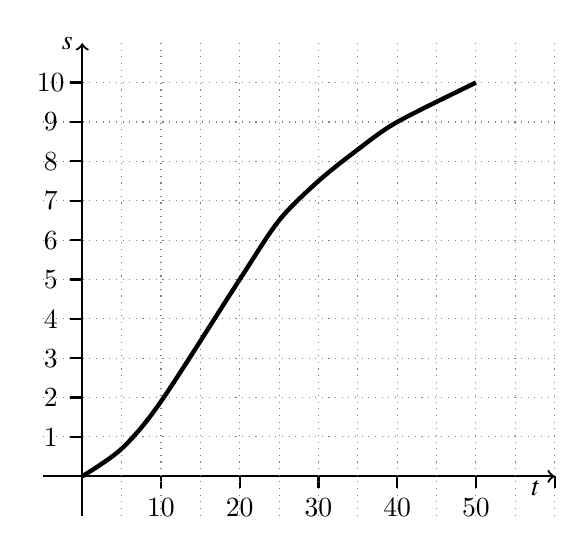
\begin{tikzpicture}[scale=.5]
\draw[thick,->] (-1,0)--(12,0);
\draw[thick,->] (0,-1)--(0,11);
\node at (-.4,11){$s$};
\node at (11.5,-0.3){$t$};
\foreach \i in {1,2,3,4,5,6,7,8,9,10}{
	\draw[dotted,thin,color=gray] (-1,\i) -- (12,\i);
	\draw[thick] (0,\i) -- (-0.3,\i);
	\node at (-.8,\i){\i};		
	}
\foreach \i in {1,2,3,4,5,6}{
	\draw[dotted,thin,color=gray] (\i,-1) -- (\i,11);
	\draw[dotted,thin,color=gray] (\i+6,-1) -- (\i+6,11);
	\draw[thick] (2*\i,0) -- (2*\i,-0.3);	
	}
\foreach \i in {10,20,30,40,50}{
	\node at (\i/5,-.8){\i};
}
\draw[ultra thick, black, smooth] plot coordinates {(0,0)(1,0.7)(2,1.9)(4,5) (5,6.5)(6,7.5)(7,8.3)(8,9)(10,10)};
\end{tikzpicture}
\end{center}
\begin{enumerate}
\item Draw the secant line between the points when $t=20$ to $t=50$ and find the slope of this line. 
\vfill
\item What does the slope from part (a) represent in the context of the problem? Include units with your answer.
\vfill
\item Describe what $s'(t)$, the derivative of $s(t)$, represents in the context of the problem and describe how it behaves as $t$ increases. 
\vfill 

\item Estimate when the runner was running the fastest and explain how you drew this conclusion.
\vfill
\end{enumerate}
\newpage
\item (15 points) Evaluate the following limits. Show your work to earn full credit. Be careful to use proper notation.
	\begin{enumerate}
	\item $\displaystyle{\lim_{x \to 2 } \frac{x^2-x-2}{2x^2-x-6}= }$
	\vfill
	\item $\displaystyle{\lim_{x \to 4^-} \frac{1+x}{\sqrt{x} +1} =}$
	\vfill
	\item $\displaystyle{\lim_{h \to 0} \frac{\frac{5}{x+h}-\frac{5}{x}}{h}= }$
	\vfill
	\end{enumerate}
\newpage
\item (15 points) Find the derivative of each function below. You do not need to simplify your answer. Be careful to appropriately parenthesize your answer.
	\begin{enumerate}
	\item $f(x)=6x^{1/2}-8x^2+\pi^{1/2}$
	\vfill
	\item $g(x)=x^4\sin(x)$
	\vfill
	\item $H(q)=\frac{q+3}{q^3+4q-2}$
	\vfill
	\end{enumerate}

\end{enumerate}
\textbf{Extra Credit:} (5 points) Use a theorem we have learned about in class to prove that there exists a solution to the equation $2^x=-2x.$ A complete answer requires some calculations \emph{and} complete sentences justifying your conclusion.
\vspace{2.5in}
\end{document}

%%%%ENDDOCUMENT


